% ! TeX root = ../../thesis.tex
\chapter{Contesto e motivazioni}
\label{chapter:context-and-motivations}

Negli ultimi decenni, con la rapida crescita di dati e informazioni facilmente accessibili sul \textit{web}, è diventato sempre più semplice poter utilizzare, in parte o in tutto, le risorse reperite.
%
Tuttavia, l'uso improprio di tali risorse e il loro appropriamento senza attribuire i necessari crediti agli autori, in violazione della legge sul \textit{copyright}, costituisce un \textbf{plagio} \cite{britannica} che, oltre ad essere una pratica scorretta che contravviene a qualsiasi ordine deontologico, rappresenta un illecito punito a norma di legge \cite{copyright-law-italia}.

Tra tutte, le due tipologie di plagio più comuni sono i plagi testuali, ovvero quelli commessi in documenti scritti in linguaggio naturale, e quelli del codice sorgente, che riguardano progetti \textit{software}, su cui verte la trattazione di questa tesi.

\section{Il problema del plagio nel software}
Anche nel mondo dell'informatica il problema del plagio è un fenomeno in crescita, incoraggiato per lo più dalla sempre maggiore quantità di progetti \textit{software} \textit{open source}, che induce gli sviluppatori a copia incollare frammenti di codice, talvolta neppure conoscendo le relative condizioni e termini di licenza.

Prima di addentrarci nell'analisi dei metodi e delle tecnologie utilizzate per l'identificazione di plagi nel contesto dei progetti informatici, è di fondamentale importanza fornire una visione d'insieme sulle strategie che vengono impiegate da parte degli sviluppatori per cercare di offuscare la copiatura quando questa è un atto deliberato.

In generale, non è possibile classificare tutti i possibili metodi con cui un programma può essere trasformato in un altro mantenendo inalterate le sue funzionalità.
%
Tuttavia, è possibile distinguere due macro categorie di modifiche: \textbf{lessicali} e \textbf{strutturali} \cite{joy-99}.

Le modifiche lessicali sono quelle che, in linea di principio, possono essere eseguite da un \textit{text editor} e non richiedono la conoscenza del linguaggio di programmazione con cui è stato sviluppato il codice.
%
Alcuni casi esemplificativi sono:
\begin{itemize}
    \item la riformulazione di commenti, la loro aggiunta o rimozione;
    \item la riformattazione del testo, come l'introduzione di spazi vuoti, di nuove linee o il cambio dell'ordine dei parametri nella definizione delle funzioni;
    \item cambiare il nome degli identificatori e delle funzioni o i tipi di dato: ad esempio da \texttt{int} a \texttt{Integer} o da \texttt{float} a \texttt{double}.
\end{itemize}

Le modifiche strutturali sono invece fortemente dipendenti dal linguaggio di programmazione e richiedono un maggior sforzo in termini di comprensione della logica del codice.
%
Di seguito alcuni esempi di rifattorizzazioni che rientrano in questa classe:
\begin{itemize}
    \item aggiungere istruzioni ridondanti, come dichiarazioni, inizializzazioni, istruzioni di stampa;
    \item sostituire i costrutti di loop con costrutti equivalenti: passare da \texttt{for} a \texttt{do/while}, o da un approccio iterativo a uno funzionale, ad esempio tramite l'uso degli \texttt{Stream} in Java;
    \item sostituire istruzioni \texttt{if} nidificate con dichiarazioni equivalenti, ad esempio \texttt{switch-case} o \texttt{when} in Kotlin, e viceversa;
    \item cambiare l'ordine di istruzioni indipendenti;
    \item cambiare l'ordine degli operandi: ad esempio \texttt{x < y} può essere cambiato in \texttt{y >= x};
    \item sostituire la chiamata a funzione con il corpo della stessa.
\end{itemize}

In \Cref{img:01-levels-of-plagiarism} viene riportata la tassonomia dei livelli di plagio di Faidhi \& Robinson definita in \cite{faidhi-robinson-1987} che mappa le possibili rifattorizzazioni in sette livelli o categorie, sulla base della loro difficoltà: il più semplice è il livello zero che corrisponde a una copia letterale; il più impegnativo è il sesto livello che corrisponde a un cambiamento logico e può essere considerato plagio solo se si verifica in concomitanza con altri livelli.

\begin{figure}[h]
    \centering
    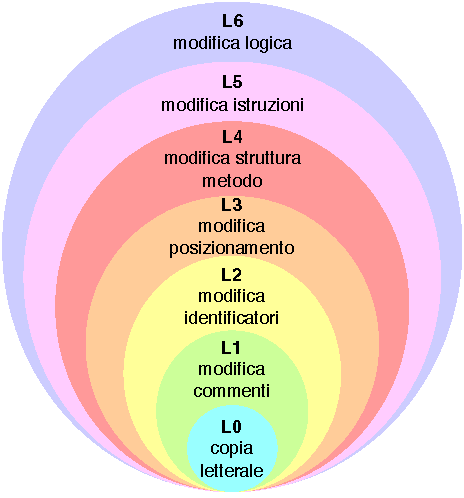
\includegraphics[width=0.55\textwidth]{resources/img/01-levels-of-plagiarism.pdf}
    \caption{Tassonomia dei livelli di plagio di Faidhi \& Robinson (1987).}
    \label{img:01-levels-of-plagiarism}
\end{figure}

Un qualunque sistema di rilevamento di plagi, perché possa essere considerato robusto ed efficace, dovrà tener conto di queste possibili rifattorizzazioni in fase di esecuzione.

\section{Sistemi antiplagio automatici}
\label{01:automatic-plagiarism-detector}
A causa dell'elevato volume di dati e informazioni disponibili che oggigiorno si hanno a disposizione, l'approccio tradizionale al rilevamento di codice copiato attraverso un'ispezione manuale, oltre che essere tedioso, è nei fatti impraticabile e, nel corso degli anni, è stato necessario porsi il problema di sviluppare strumenti di rilevamento automatici di plagi che siano efficienti ed efficaci.
%
Ciononostante, un'ispezione manuale a seguito di quella automatica è tuttora ancora necessaria per stabilire con ragionevole certezza se le porzioni di codice individuate dal sistema sono effettivamente copiature o, più ingenuamente, blocchi simili di codice.

Più formalmente, detto $p = \{s_{plg}, d_{plg}, s_{src}, d_{src}\}$ un caso di plagio, $s_{plg}$ un passaggio del documento $d_{plg}$ che è copiato a partire da un passaggio $s_{src}$ in un documento $d_{src}$, il compito di un sistema automatico di rilevamento di plagi consiste nell'individuare la tupla $p$ \cite{yalcin-et-al-2022}.

Già a partire dagli anni settanta del novecento, sono stati proposti algoritmi e tecniche per l'analisi del codice, nonché l'identificazione e localizzazione di sezioni simili di sorgenti.

In questo contesto è da porre in evidenza la differenza tra l'individuazione di cloni e quella di plagi.
%
Quando ci si riferisce a un clone, infatti, lo si fa con riferimento a un frammento di codice che è stato copiato e marginalmente modificato. 
%
Quando invece ci si riferisce ad un plagio si intende una sezione che è stata copiata e la cui opera di copiatura si è cercato di dissimulare, mediante opportune azioni di rifattorizzazione del codice \cite{cpdp}, descritte nel paragrafo precedente.
%
Dunque, l'ambito di applicazione delle due ricerche è nettamente diverso: se nel primo l'obiettivo è quello di evidenziare il codice duplicato al fine di migliorare la qualità del codice e la manutenibilità del sistema, nel secondo lo scopo primario è identificare possibili condotte illecite.

Questo aspetto è, insieme alle prestazioni, la sfida principale da affrontare durante la progettazione di un sistema antiplagio.

Gli strumenti d'identificazione di plagi devono infatti cercare di annullare gli effetti di queste rifattorizzazioni.
%
Maggiore sarà il livello di rifattorizazzione a cui il sistema sarà insensibile, migliore sarà l'efficacia e la robustezza del sistema stesso.
%
A questo scopo le tecniche di analisi si compongono di più fasi nelle quali trasformano i sorgenti in rappresentazioni intermedie che astraggono il più possibile dai dettagli implementativi, che possono essere facilmente cambiati, quindi applicano su di esse tecniche di confronto.

Si osservi, tuttavia, che esistono rifattorizzazioni il cui contributo è più facile da annullare di altre. 
%
Si pensi, ad esempio, all'aggiunta o alla modifica dei commenti: l'effetto di tale rifattorizzazione è facilmente annullabile semplicemente trascurando dall'analisi i commenti, in quanto non contribuiscono in alcun modo alla logica del programma. 
%
D'altro canto, creare tecniche che siano insensibili al riordino delle istruzioni è un compito più complesso, fonte di approfonditi studi e ambito di ricerca.

L'altro problema emergente nello sviluppo di un programma antiplagio che non si limiti a confrontare la similarità tra una coppia di progetti, bensì effettui un controllo uno a molti o molti a molti, in cui si testano tutte le possibili coppie, sono le prestazioni. 
%
Infatti, la maggioranza delle tecniche e degli algoritmi per effettuare i confronti sono inefficienti in termini di tempo costo. 
%
Questo è in larga parte dovuto al fatto che la misurazione della somiglianza tra una coppia di sorgenti, nella gran parte degli algoritmi noti in letteratura, ha una complessità almeno quadratica nel numero delle istanze delle sue rappresentazioni, e che, per ogni valutazione, il numero di confronti da effettuare è tipicamente elevato: detto $N$ il numero di progetti, volendo confrontare tutte le coppie di progetti tra loro, dovrebbero essere eseguite $\frac{N(N-1)}{2}$ comparazioni.
%
Questo problema è acuito inoltre dal fatto che i progetti \textit{software} stanno diventando sempre più complessi e si hanno a disposizione una sempre maggior quantità di dati da dover processare.

Per questa ragione vengono sfruttate tecniche di parallelizzazione e devono essere adottate strategie di ottimizzazione in grado di ridurre il numero di confronti da effettuare e, quindi, diminuire il tempo di esecuzione.
%
Per farlo, si utilizzano tecniche euristiche che permettono di determinare il grado di somiglianza dei sorgenti senza dover effettivamente eseguire il confronto.

Va da sé che l'utilizzo di tali tecniche impatta inevitabilmente la sensibilità del sistema: una stima errata, a monte, della somiglianza di due sorgenti può portare a non effettuare alcun confronto tra questi e quindi a non individuare possibili plagi. 
%
Questo si verifica soprattutto nei casi in cui l'ottimizzazione è molto marcata e si riduce in modo eccessivo l'insieme dei sorgenti su cui effettuare il confronto, rendendo di fatto svantaggioso l'impiego di tali tecniche.

Il bilanciamento tra le prestazioni e l'efficacia del sistema è, dunque, di fondamentale importanza.

\section{Stato dell'arte}
Il codice sorgente non è nient'altro che un file di testo scritto da sviluppatori, che deve essere compilato o interpretato e che, pertanto, si basa su regole sintattiche e grammaticali proprie del linguaggio di programmazione con cui è scritto che permettono a entrambi gli attori, il programmatore e il calcolatore, di "capirlo" ed elaborarlo.
%
Per questo motivo, se processare la struttura di un sorgente non presenta grandi difficoltà, processare il significato, ovvero l'idea e la logica sottesa al codice, costituisce una sfida più grande, se non altro perché entra in gioco la competenza dello sviluppatore e la sua esperienza nella scrittura di codice "pulito".

Poiché il problema è complesso, gli attuali metodi analizzano il codice sorgente utilizzando un particolare "punto di vista", alcuni cercando di comprenderne il significato, altri la loro struttura.
%
Con lo sviluppo della tecnologia, molti ricercatori hanno fatto progressi in questo campo e proposto diversi algoritmi, formando gradualmente tre popolari famiglie di tecniche: \textbf{\textit{attribute-based}}, \textbf{\textit{structure-based}} e \textbf{tecniche ibride} \cite{es-plag}.

\subsection{Analisi \textit{attribute-based}}
Il primo sistema automatico di rilevazione di codice copiato che sia stato documentato in letteratura risale al 1976 \cite{ottenstein} ed era basato sulle seguenti quattro metriche di Healstead per determinare il livello di similarità tra coppie di sorgenti \cite{halstead}:

\begin{itemize}
    \item $\eta_1$: il numero di operatori univoci;
    \item $\eta_2$: il numero di operandi univoci;
    \item $N_1$: il numero di occorrenze di un operatore;
    \item $N_2$: il numero di occorrenze di un operando.
\end{itemize}

Coppie di sorgenti con valori identici per ciascuna di queste metriche si presumeva fossero simili e meritevoli di un esame più approfondito.

Nel corso degli anni, sono state proposte altre metriche per ottenere stime sempre più accurate di somiglianza e per riflettere sempre più la struttura del flusso di controllo del programma, come il numero d'istruzioni di \textit{loop} e di espressioni condizionali, il numero di procedure e di istruzioni di \textit{input}, il numero medio di caratteri per linea e altre ancora \cite{pdectet}.

Collettivamente, questi sistemi sono stati definiti \textit{attribute counting metric systems} in quanto fondano il confronto sull'analisi di metriche basate su attributi intrinseci del codice sorgente.

Tuttavia, considerando che le caratteristiche del codice sorgente non sono strettamente correlate alla semantica del programma e che la misurazione della somiglianza può risultare essere imprecisa, l'efficacia di queste tecniche è considerevolmente limitata in termini di accuratezza se confrontata con quella di tecniche \textit{structure-based} \cite{es-plag}.

\subsection{Analisi \textit{structure-based}}
Le tecniche di analisi \textit{structure-based}, a differenza di quelle \textit{attribute-based}, si basano, come suggerisce il nome stesso, sulla struttura dei codici sorgenti per determinare il grado di similarità tra gli stessi.

Nella maggioranza dei casi, i sistemi che implementano questo tipo di tecnica lavorano in due fasi consecutive: prima il codice sorgente viene analizzato e viene generata una rappresentazione intermedia, poi si effettua il confronto dei sorgenti sulle rappresentazioni intermedie.

All'interno di questo tipo di analisi possiamo annoverare principalmente due diversi metodi: l'analisi lessicale e quella basata su un modello astratto e derivato dai sorgenti.

\subsubsection{Analisi lessicale (\textit{tokenizzazione})}
\label{01-tokenization}

Tra tutte, la tecnica più usata è l'analisi lessicale del codice sorgente (\textbf{\textit{lexical analysis}} o \textbf{\textit{tokenization}} in inglese), che consiste nel convertire la sequenza di caratteri di cui è composto il programma in una sequenza di \textit{token}.
%
Un \textit{token} è, a sua volta, un simbolo astratto che rappresenta un tipo di unità lessicale nella grammatica del linguaggio. 
%
Esso è associato a un \textbf{lessema}, ovvero ad una sequenza di caratteri del programma che corrisponde al \textit{pattern} di un \textit{token} identificato dall'analizzatore lessicale come una specifica istanza di quel \textit{token}, e da attributi opzionali derivati dal testo.
%
Alcuni possibili esempi di \textit{token} comuni con i relativi \textit{pattern} e alcuni lessemi di esempio sono riportati in \Cref{table:token-examples}.

\begin{table}[h]
    \centering
    \begin{tabular}{|p{0.15\linewidth}|p{0.45\linewidth}|p{0.3\linewidth}|}
        \hline
        \textbf{\textit{Token}} & \textbf{Pattern} & \textbf{Lessemi di esempio} \\ [0.5ex] 
        \hline\hline
        \textit{identifier} & Stringa di lettere e numeri che iniziano con una lettera & \texttt{x}, \texttt{name}, \texttt{color}, ... \\ 
        \hline
        \textit{keyword} & Coincide con la sequenza di caratteri della \textit{keyword} stessa & \texttt{if}, \texttt{for}, \texttt{return}, ... \\
        \hline
        \textit{literal} & Ogni stringa racchiusa tra virgolette ("") tranne la stringa nulla '' & \texttt{"Hello World!"}, ... \\
        \hline
        \textit{operator} & "\texttt{<}", "\texttt{>}", "\texttt{<=}", "\texttt{>=}", "\texttt{==}" "\texttt{!=}" & \texttt{<=}, \texttt{!=}, ... \\
        \hline
    \end{tabular}
    \caption{Esempi di possibili \textit{token} comuni.}
    \label{table:token-examples}
\end{table}

L'analisi lessicale rappresenta il primo stadio della struttura di un compilatore ed è eseguita da programmi denominati \textbf{\textit{lexer}}. 
%
Questi sono generati in maniera dichiarativa a partire da generatori di \textit{lexer} (\textbf{\textit{lexer generator}}) che, presi in input più automi a stati finiti, espressi per mezzo di espressioni regolari che definiscono in maniera formale la grammatica del linguaggio, generano il codice che implementa l'algoritmo di analisi lessicale. 
%
In \Cref{img:01-id-finite-automa} è mostrato un esempio di automa a stati finiti che riconosce un identificatore.
%
L'equivalente espressione regolare è la seguente: \texttt{[a-zA-Z].([a-zA-Z]|[0-9])*}.

\begin{figure}[h]
    \centering
    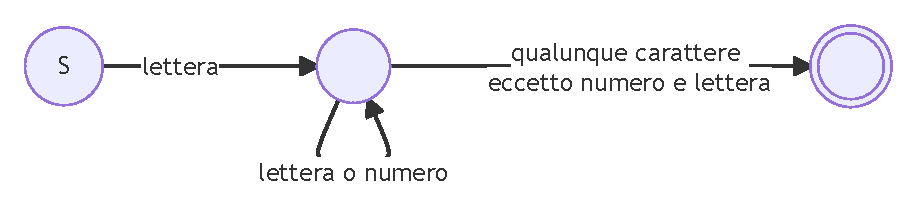
\includegraphics[width=0.8\textwidth]{resources/img/01-id-finite-automa.pdf}
    \caption{Esempio di automa a stati finiti che riconosce un identificatore.}
    \label{img:01-id-finite-automa}
\end{figure}

Attraverso questo approccio, quindi, ogni programma viene trasformato in una sequenza di \textit{token}, uno per ciascun elemento di base del linguaggio che si vuole valorizzare: le sezioni di codice non rilevanti ai fini della comparazione possono essere escluse, cioè non viene generato alcun \textit{token} per questi elementi.

In \Cref{table:token-associations} è mostrata una possibile sequenza di \textit{token} generata a partire dalla classe presentata nel \Cref{lst:test-analysis}.
%
Il risultato che si ottiene è una versione condensata e semplificata del sorgente, con un vocabolario ristretto, in cui le dichiarazioni superflue, come quelle di \texttt{import}, \texttt{package} e il blocco di documentazioni, sono ignorati.

\lstinputlisting[
    float,
 	language=Java,
 	caption={Una semplice classe che stampa su \textit{console} gli argomenti passati in \textit{input}, se presenti, o un saluto, per mostrare il processo di \textit{tokenizzazione}},
 	label={lst:test-analysis},
]{resources/code/01-TestAnalysis.java}

\begin{table}[h!]
    \centering
    \begin{tabular}{|c|c|c|} 
        \hline
        \textbf{Linee} & \textbf{Costrutto} & \textbf{\textit{Token}} \\ [0.5ex] 
        \hline\hline
        1   & \texttt{package}                    & \texttt{-}                            \\ \hline
        3   & \texttt{import}                     & \texttt{-}                            \\ \hline
        5-7 & \texttt{/** This is ... process.*/} & \texttt{-}                            \\ \hline
        8   & \texttt{public}                     & \texttt{-}                            \\ \hline
        8   & \texttt{class}                      & \texttt{ClassOrInterfaceDeclaration}  \\ \hline
        8   & \texttt{Main}                       & \texttt{Identifier}                   \\ \hline
        8   & \texttt{\{}                         & \texttt{-}                            \\ \hline
        9   & \texttt{public}                     & \texttt{Modifier}                     \\ \hline
        9   & \texttt{static}                     & \texttt{Modifier}                     \\ \hline
        9   & \texttt{void}                       & \texttt{VoidType}                     \\ \hline
        9   & \texttt{main}                       & \texttt{Identifier}                   \\ \hline
        9   & \texttt{String[]}                   & \texttt{ArrayType}                    \\ \hline
        9   & \texttt{args}                       & \texttt{Identifier}                   \\ \hline
        9   & \texttt{\{}                         & \texttt{-}                            \\ \hline
        10  & \texttt{if}                         & \texttt{IfStmt}                       \\ \hline
        10  & \texttt{args.length}                & \texttt{FieldAccessExpr}              \\ \hline
        10  & \texttt{>}                          & \texttt{Operator}                     \\ \hline
        10  & \texttt{0}                          & \texttt{IntegerLiteralExpr}           \\ \hline
        10  & \texttt{\{}                         & \texttt{-}                            \\ \hline
        11  & \texttt{System.out.println}         & \texttt{MethodCallExpr}               \\ \hline
        11  & \texttt{"Program arguments"}        & \texttt{StringLiteralExpr}            \\ \hline
        11  & \texttt{Arrays.toString}            & \texttt{MethodCallExpr}               \\ \hline
        11  & \texttt{args}                       & \texttt{NameExpr}                     \\ \hline
        11  & \texttt{\}}                         & \texttt{-}                            \\ \hline
        12  & \texttt{else}                       & \texttt{elseStmt}                     \\ \hline
        12  & \texttt{\{}                         & \texttt{-}                            \\ \hline
        13  & \texttt{System.out.println}         & \texttt{MethodCallExpr}               \\ \hline
        13  & \texttt{"Hello world ... Java!"}    & \texttt{StringLiteralExpr}            \\ \hline
        14-16  & \texttt{\}}                         & \texttt{-}                            \\ \hline
    \end{tabular}
    \caption{Associazioni costrutti-\textit{token} del \Cref{lst:test-analysis}}
    \label{table:token-associations}
\end{table}

Questo approccio rende il sistema sufficientemente robusto contro semplici tecniche di \textit{refactoring}, come la modifica degli identificatori, corrispondente al secondo livello della tassonomia di Faidhi \& Robinson (\Cref{img:01-levels-of-plagiarism}).

Tuttavia, bisogna evidenziare come l'efficacia della \textit{tokenizzazione} dipende dall'insieme di \textit{token} che si decide di usare.
%
Consideriamo, a puro scopo esemplificativo, il caso delle \textit{keyword} dedicate a rappresentare un intero in Java.
%
Come sappiamo, un intero è rappresentabile con diversi tipi di dato; a seconda delle esigenze di memoria, infatti, si potrebbe usare, considerando solo i tipi di dato primitivo e tralasciando quelli \textit{boxed}, un \texttt{byte}, piuttosto che uno \texttt{short}, un \texttt{int} o un \texttt{long}. 
%
Un insieme "stringente" di \textit{token} potrebbe rappresentare ciascuno di questi tipi con un proprio \textit{token}.
%
D'altro canto, un set di \textit{token} "lasco" potrebbe rappresentare tutti e quattro i tipi di dato sopra citati con un unico \textit{token}, riconoscendo che tutti e quattro possono servire, nella grande maggioranza dei casi, allo stesso scopo.
%
Pertanto un insieme di \textit{token} "lasco" aiuta il sistema a riconoscere e catalogare come equivalenti tipi di dato diversi e fornire quindi una maggiore resilienza alle tecniche di rifattorizzazione.

Spesso, la fase di analisi lessicale è seguita da una fase di filtraggio, che consente di ridurre il numero di rappresentazioni da dover confrontare e, quindi, il numero stesso dei confronti, portando a una riduzione dei tempi di esecuzione.
%
Questo stadio è preceduto da una fase d'indicizzazione in cui, a partire dalla sequenza di \textit{token}, vengono generati alcuni indici, ovvero strutture che raggruppano i dati e che permettono di inferire una stima euristica della similarità, senza dover effettuare il confronto \textit{token} per \textit{token}.
%
Una tra gli indici più comuni è costituito da coppie chiave$-$valore in cui nelle chiavi sono memorizzati i tipi di \textit{token} e nei valori la loro frequenza, in termini di numero di occorrenze all'interno del sorgente.
%
Un esempio di indice costruito a partire dalla sequenza di \textit{token} elencata in \Cref{table:token-associations} è mostrato in \Cref{table:token-indexing}.
%
\begin{table}[h!]
    \centering
    \begin{tabular}{|c|c|} 
        \hline
        \textbf{Tipo di \textit{token}} & \textbf{Frequenza} \\ [0.5ex] 
        \hline\hline
        \texttt{ClassInterfaceDeclaration}  & 1 \\ \hline
        \texttt{Identifier}                 & 3 \\ \hline
        \texttt{Modifier}                   & 2 \\ \hline
        \texttt{VoidType}                   & 1 \\ \hline
        \texttt{ArrayType}                  & 1 \\ \hline
        \texttt{IfStmt}                     & 1 \\ \hline
        \texttt{FieldAccessExpr}            & 1 \\ \hline
        \texttt{Operator}                   & 1 \\ \hline
        \texttt{IntegerLiteralExpr}         & 1 \\ \hline
        \texttt{MethodCallExpr}             & 3 \\ \hline
        \texttt{NameExpr}                   & 1 \\ \hline
        \texttt{elseStmt}                   & 1 \\ \hline
        \texttt{StringLiteralExpr}          & 2 \\ \hline
    \end{tabular}
    \caption{Indice con coppie (tipo di \textit{token}$-$frequenza) generate a partire dalla \Cref{table:token-associations}}
    \label{table:token-indexing}
\end{table}
%
Tali indici sono successivamente impiegati nella vera e propria fase di filtraggio in cui viene applicata una particolare metrica, ad esempio la similarità coseno, per escludere le coppie di sorgenti con similarità inferiore ad un valore di soglia, scelto coerentemente alla metrica.

A seguire i sorgenti vengono confrontati con algoritmi di \textit{string matching}.
%
Tra questi, i due più conosciuti sono \textbf{\textit{Winnowing}} \cite{winnowing} e \textbf{\textit{Running-Karp-Rabin Greedy String Tiling (RKR-GST)}} \cite{wise-running-93}.

\textit{Winnowing} costituisce un miglioramento della tecnica nota come \textit{k-gram fingerprinting} e consiste nei seguenti passi:
\begin{itemize}
    \item il documento viene suddiviso in una lista di sottostrighe di lunghezza $k$, denominati \textit{k-grams};

    \item grazie all'utilizzo di un'opportuna funzione di \textit{hashing} ciascun \textit{k-gram} è trasformato in un valore numerico;
    
    \item la sequenza numerica è trasformata in una sequenza di "finestre" di valori di \textit{hash}, in cui la grandezza di ciascuna, detta $w$, è data da: $w = t - n + 1$ dove $t$ rappresenta la lunghezza minima delle stringhe che è garantito siano trovate e $n$ rappresenta la lunghezza massima delle stringhe che è garantito \textit{non} siano trovate;
    
    \item sono selezionati un sottoinsieme dei valori di \textit{hash}, da usare come impronta digitale del documento, considerando il valore minimo di ogni finestra di valori.
\end{itemize}

La comparazione avviene successivamente sulla base di queste "impronte digitali", che sono dimostrate essere rappresentative della struttura del documento \cite{winnowing}.
%
In \Cref{img:01-winnowing-example} è presentato un esempio tratto da \cite{winnowing} in cui vengono mostrati i passi dell'algoritmo applicati a una semplice stringa di caratteri.

\begin{figure}[h!]
    \centering
    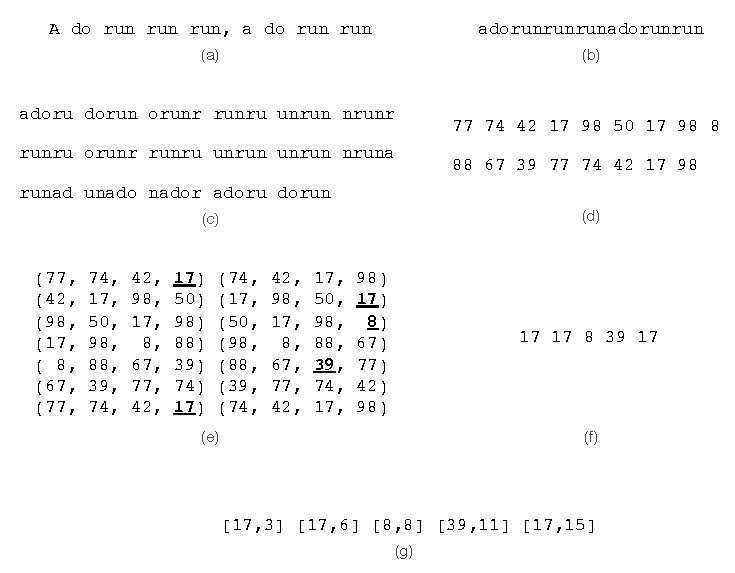
\includegraphics[width=\textwidth]{resources/img/01-winnowing-example.pdf}
    \caption[Passi esemplificativi dell'algoritmo \textit{Winnowing} applicati a un semplice testo scritto in linguaggio naturale.]{Passi esemplificativi dell'algoritmo \textit{Winnowing} applicati a una semplice sequenza di caratteri. In $(b)$ le caratteristiche irrilevanti sono state rimosse (virgole, spazi) e in $(c)$ la sequenza di caratteri è trasformata in una sequenza di \textit{5-gram}. In $(d)$ è mostrata una possibile sequenza risultante dell'applicazione di una funzione di \textit{hashing}. A partire da tale sequenza viene creata una sequenza di "finestre" di lunghezza 4, da ciascuna delle quali è selezionato il valore di \textit{hash} minore (in grassetto sottolineato) avendo cura di non selezionare più volte lo stesso valore a causa della sovrapposizione delle finestre $(f)$. Infine, in $g$,  ciascun valore di \textit{hash} selezionato viene accoppiato con l'indice \textit{0-based} della sua posizione al passo $(d)$.}
    \label{img:01-winnowing-example}
\end{figure}

\textit{Running-Karp-Rabin Greedy String Tiling (RKR-GST)} costituisce l'altra popolare alternativa a \textit{Winnowing}, che tenta di aumentare la sua precisione a discapito dell'efficienza. 
%
Esso incorpora, di fatto, due algoritmi.
%
\textit{Greedy String Tiling (GST)} è l'algoritmo che trova la massima sottosequenza comune in due stringhe.
%
\textit{Running-Karp-Rabin (RKR)} è l'algoritmo per la ricerca rapida di sottosequenze comuni e trova tutte le occorrenze di una stringa $P$ all'interno di una stringa più lunga $T$ effettuando l'\textit{hashing} di tutte le sottostringhe di lunghezza $|P|$ e confrontandole con gli \textit{hash} di $P$.
%
I due algoritmi cooperano in questo modo: \textit{RKR} è eseguito su due programmi.
%
Per ogni sottosequenza comune identificata da \textit{RKR}, \textit{GST} è eseguito per estendere il \textit{match} rintracciato mediante l'uso della funzione di \textit{hashing}.
%
I dettagli e lo pseudocodice dell'algoritmo sono descritti nella \Cref{03-matching-algorithms}.

\subsubsection{Analisi basata su un modello}
Anziché utilizzare la sequenza di \textit{token} generata dal \textit{lexer} possono essere generate delle strutture e dei modelli più complessi, che permettano di astrarre ulteriormente dalla sintassi del linguaggio.

Una tra le rappresentazioni più note e naturali in questo ambito, derivata dalla stessa analisi lessicale, è l'\textbf{albero sintattico} (o \textit{abstract syntax tree} in inglese, abbreviato \textit{AST}).
%
Questo è generato a partire dalla sequenza di \textit{token} descritta nel paragrafo precedente e rappresenta il risultato ottenuto a seguito dell'applicazione del secondo stadio di un compilatore: il \textbf{\textit{Parser}} (\Cref{img:01-compiler-arch}).
%
Esso, infatti, presa in \textit{input} la sequenza di \textit{token}, la converte in una struttura dati ad albero che rappresenta la struttura logica del codice sorgente.

\begin{figure}[h]
    \centering
    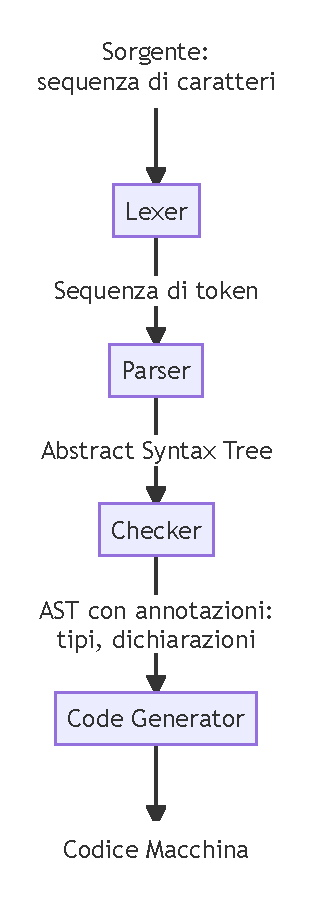
\includegraphics[width=0.2\textheight]{resources/img/01-compiler-arch.pdf}
    \caption{Struttura sommaria di un compilatore.}
    \label{img:01-compiler-arch}
\end{figure}

L'albero risultante dall'applicazione del \textit{parser} è definito "astratto" in quanto non rappresenta ogni dettaglio tipico della sintassi del linguaggio, bensì solo i dettagli strutturali e relativi al contenuto.
%
Ad esempio, le parentesi di raggruppamento sono rappresentate nativamente nella struttura ad albero, quindi non devono essere rappresentate come nodi separati.
%
Allo stesso modo, un costrutto sintattico come un'istruzione \texttt{if-then-else} può essere facilmente denotata per mezzo di un singolo nodo con tre rami.

In \Cref{img:01-ast} viene mostrata la struttura parziale dell'\textit{AST} del metodo \texttt{main()} del \Cref{lst:test-analysis}.

\begin{sidewaysfigure}
    \makebox[\textwidth][c]{
        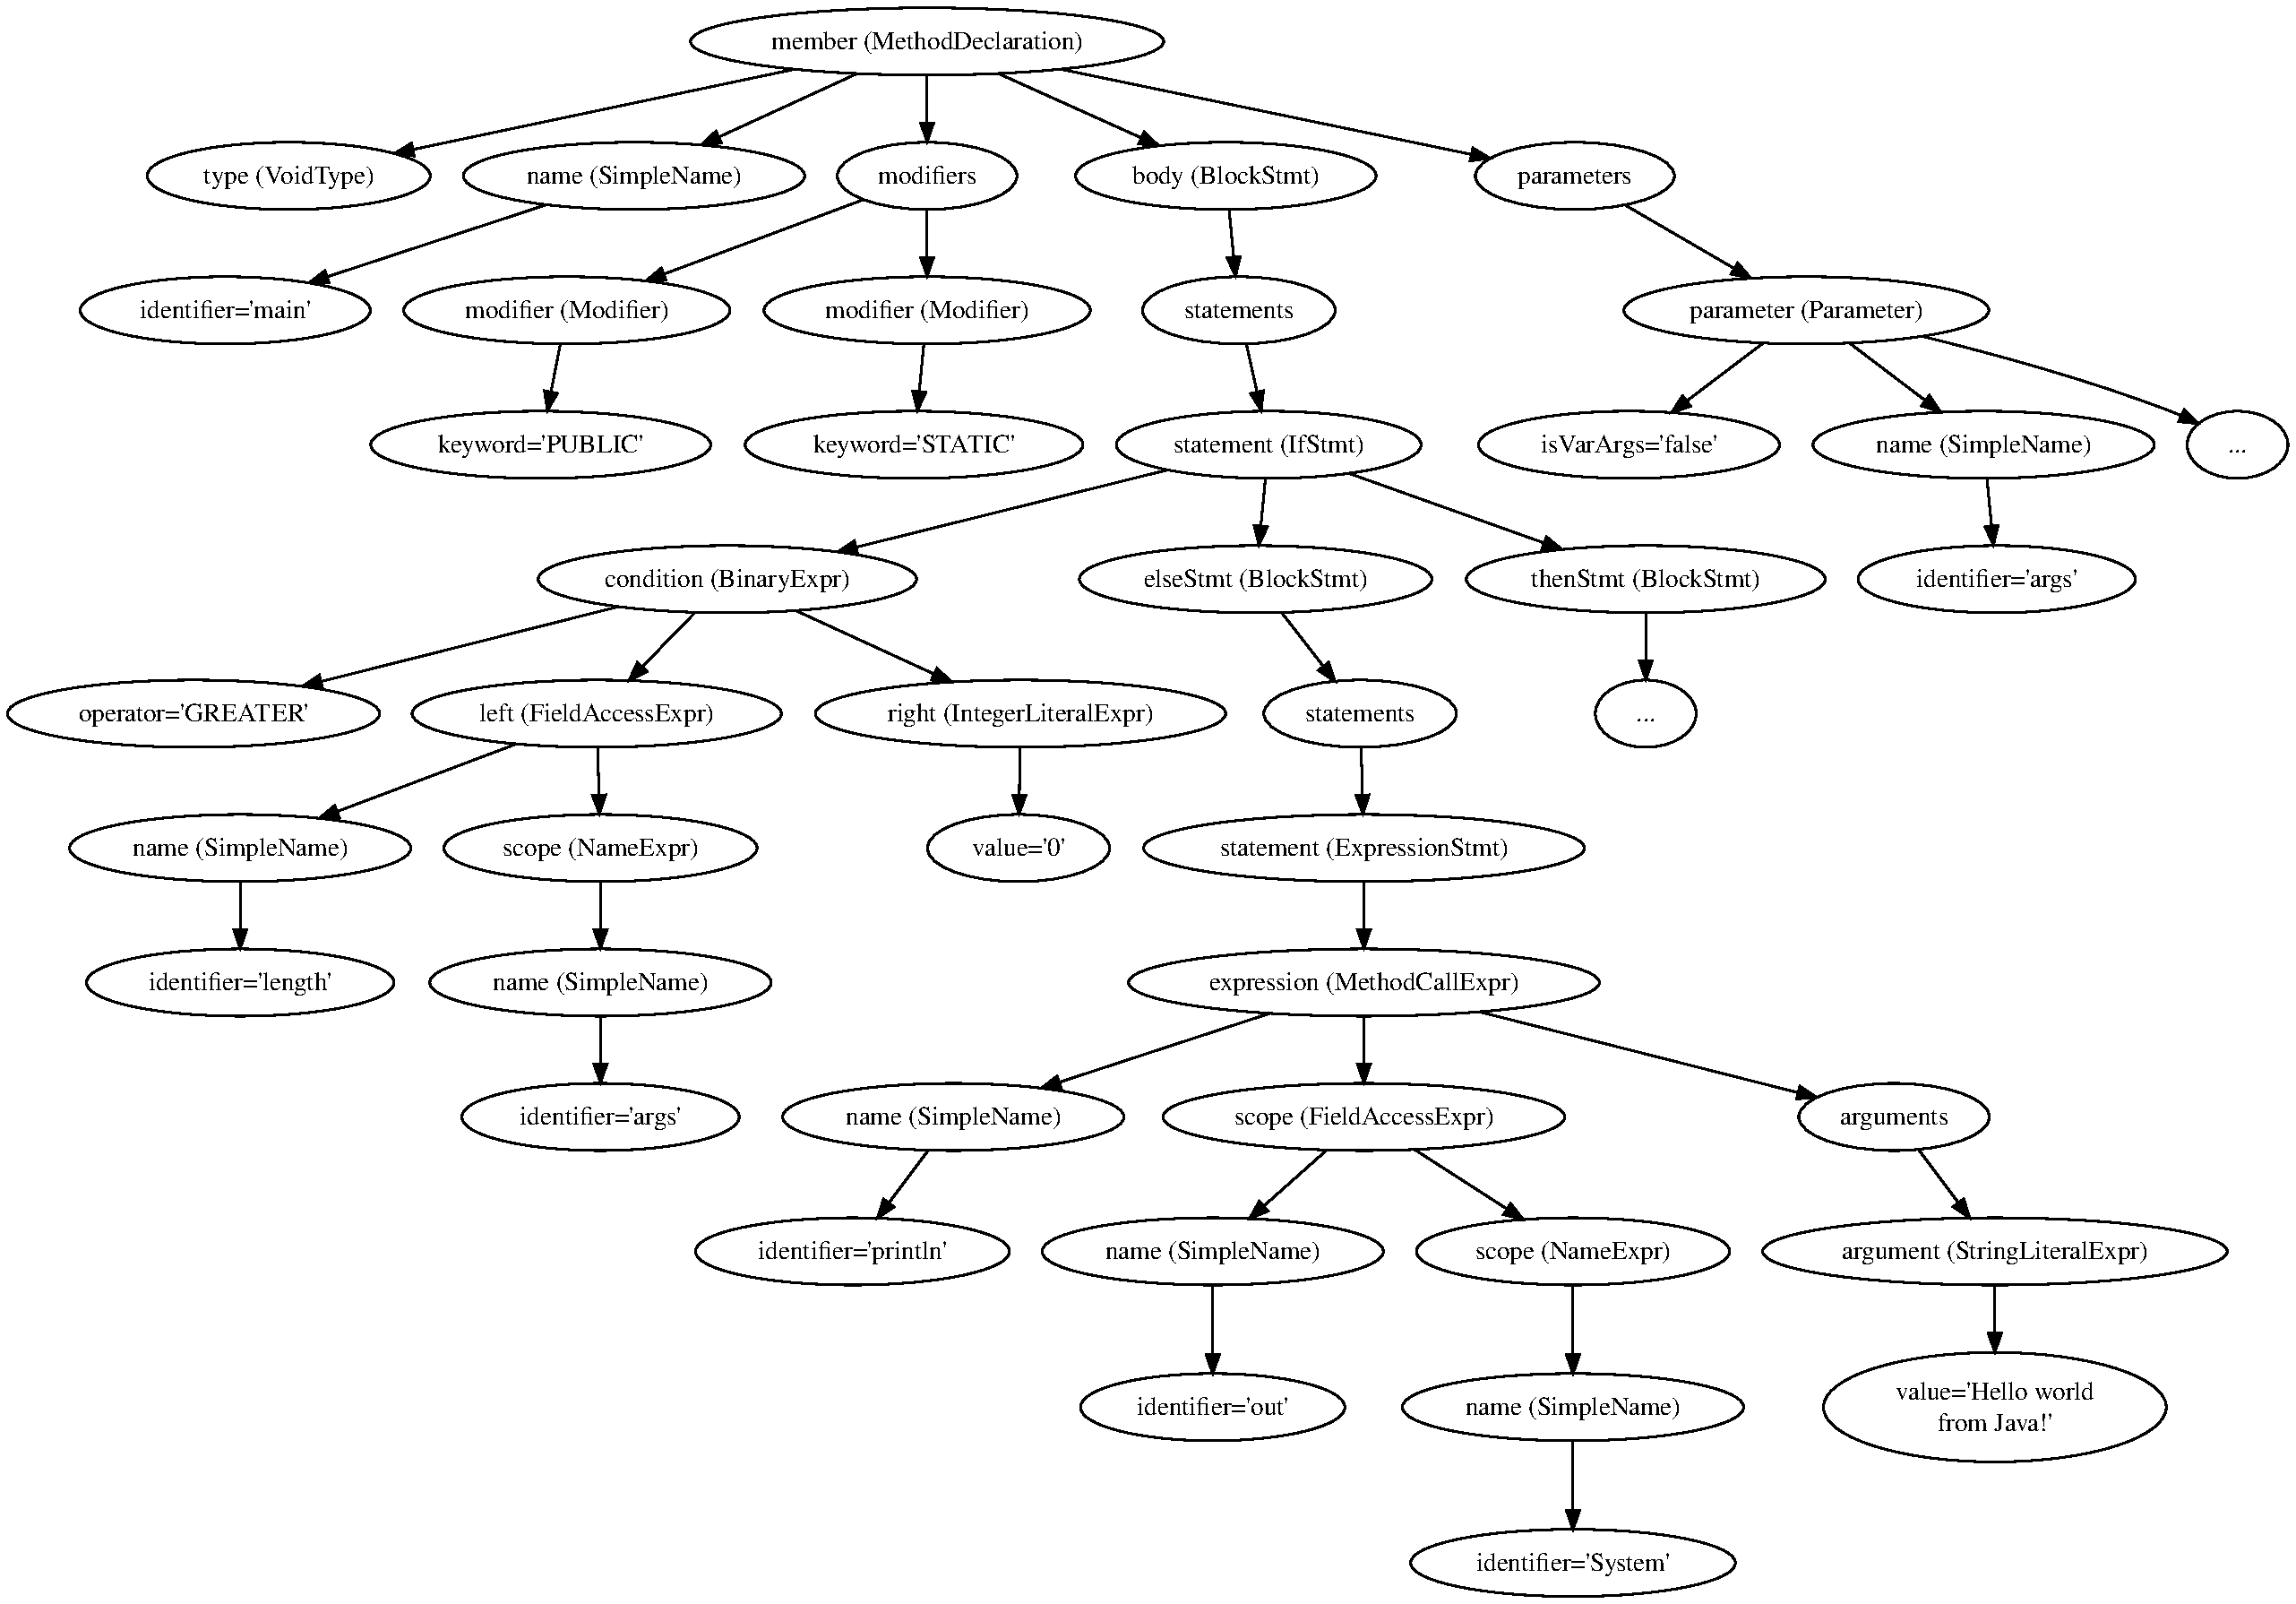
\includegraphics[width=1.1\textwidth]{resources/img/01-ast-summarized.pdf}
    }
    \caption{Rappresentazione di una porzione dell'\textit{AST} del metodo \texttt{main} del \Cref{lst:test-analysis}}
    \label{img:01-ast}
\end{sidewaysfigure}

Avere a disposizione una struttura ad albero per ciascun sorgente è di fondamentale importanza e agevola la fase di \textit{preprocessing} in cui si va "ripulire" il sorgente di tutte le sezioni non rilevanti.
%
Inoltre, il confronto dei sorgenti per mezzo di alberi sintattici fornisce risultati migliori di quelli ottenuti mediante una pura analisi lessicale del codice.
%
Il principale e non trascurabile svantaggio di utilizzare questo approccio, tuttavia, risiede nelle prestazioni.
%
Siccome la maggior parte degli AST sono strutture complesse e voluminose, la comparazione diretta degli alberi sintattici per una grande quantità di sorgenti è proibitiva.
%
Per far fronte a questo problema, per ogni albero viene determinato, mediante un'opportuna funzione di \textit{hashing} che tiene conto del tipo di ciascun nodo e del suo sotto-albero, un valore di \textit{hash} e la comparazione è effettuata confrontando tali valori.

Altri approcci sono presenti in letteratura, tra cui l'utilizzo di grafi che descrivono le dipendenze del programma, detti \textit{Program Dependency Graph}, abbreviato \textit{PDG} \cite{gplag}.
%
\textit{PDG} è una rappresentazione di una procedura del sorgente a grafo in cui le istruzioni rappresentano l'insieme dei vertici e le dipendenze di dati e di controllo tra le istruzioni rappresentano gli archi.
%
In \Cref{img:01-pdg} è mostrato un esempio, tratto da \cite{gplag}, di \textit{PDG} per le due funzioni presentate nel \Cref{lst:pdg}.
%
La comparazione tra questi avviene sfruttando l'isomorfismo di grafi\footnote{Nella teoria dei grafi l'isomorfismo di due grafi, $G$ e $H$, è una biiezione tra i loro vertici che preserva i bordi, ovvero tale che, data una coppia qualsiasi $(u, v)$ adiacente in $G$, la coppia $(f(u), f(v))$ sia ancora adiacente in $H$.}.

\lstinputlisting[
    language=c,
    caption={Due semplici funzioni, in C, che effettuanao la somma di un \textit{array} utilizzate per mostrare il corrispondente \textit{PDG}},
    label={lst:pdg}
]{resources/code/01-pdg.c}

\begin{figure}[h!]
    \makebox[\textwidth][c]{
        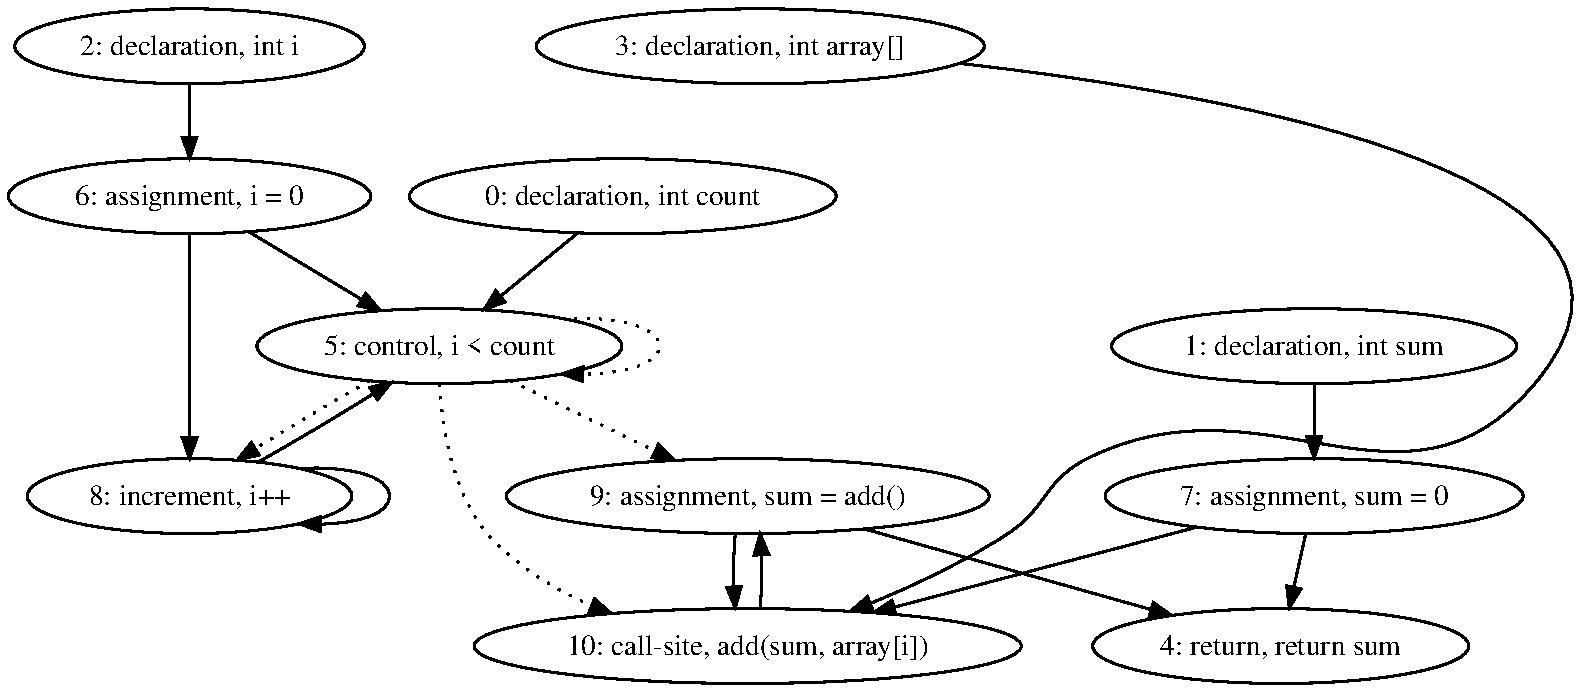
\includegraphics[width=1.1\linewidth]{resources/img/01-pdg.pdf}
    }
    \caption{Esempio di \textit{PDG} della funzione \texttt{sum} del \Cref{lst:pdg}.}
    \label{img:01-pdg}
\end{figure}

\subsection{Tecniche ibride}
Entrambi i tipi di tecniche descritti sopra hanno i loro vantaggi e svantaggi. 
%
Alcuni lavori di ricerca hanno pertanto cercato di combinare entrambi gli approcci creando, di fatto, tecniche di analisi ibride, alcune delle quali adattate da altri domini, regolando l'influenza di un approccio sull'altro sulla base delle proprie esigenze.
%
Tra queste, spiccano per importanza la \textit{Latent Semantic Analysis} \cite{lsa} e le tecniche di \textit{Clustering} \cite{pdectet}.

La prima è un metodo di elaborazione del linguaggio naturale che analizza le relazioni tra un insieme di documenti e i termini in esso contenuti: dapprima sono applicati modelli statistici che riflettono l'importanza che ciascun termine (nel caso dei sorgenti, i \textit{token}) assume in un insieme di documenti e, successivamente, attraverso l'utilizzo di una tecnica algebrica di fattorizzazione di una matrice basata sull'uso di autovalori e autovettori detta \textit{Singular Value Decomposition}, vengono trovate relazioni nascoste (latenti, da qui il nome \textit{Latent Semantic Analysis}) tra i termini e concetti.

La seconda utilizza una rappresentazione a grafo in cui i vertici rappresentano gli identificatori e gli archi (pesati) la misura di similarità tra i programmi, trasformando il problema di trovare sezioni di codice duplicati nel problema di \textit{clustering} di un grafo pesato.

Altri metodi, qui non approfonditi, sono in via di sviluppo e impiegano algoritmi di \textit{machine learning} come \textit{Random Forest} e \textit{Gradient Boosting} applicati agli alberi di regressione.

\subsection{Quale tecnica scegliere?}
In conclusione, bisogna rendersi conto che, a prescindere dal grado di sofisticatezza della tecnica che si utilizza, è sempre possibile che si verifichi un plagio non rilevabile \cite{joy-99}.
%
Il bilancimento tra le risorse investite nell'individuazione dei plagi e i rendimenti decrescenti di trovare i pochi, se non nessuno, casi difficili da rilevare è un fattore critico che necessita un'analisi approfondita, tenuto conto delle specifiche esigenze del dominio applicativo.

Stabilire quale tecnica scegliere è complesso, perché difficili da confrontare tra loro: la maggior parte di queste viene valutata utilizzando il proprio \textit{set} di dati, che raramente sono resi pubblicamente accessibili e che potrebbero non rappresentare veri casi di plagio \cite{karnalim-budi-toba-joy-2019}.

Ciononostante, le tecniche più utilizzate in questo ambito e più efficaci sulla base delle considerazioni suffatte, sono quelle \textit{structure-based}, che verranno impiegate anche nello strumento sviluppato nell'ambito di questa tesi. 
